\documentclass[11pt]{article}

% Make margins smaller
\usepackage[top=1.1in, bottom=1.1in, left=1.1in, right=1.1in]{geometry}
% more advanced mathematical symbols
\usepackage{amsfonts}
\usepackage{amssymb}
\usepackage{amsmath}
\usepackage{bm}
\usepackage{bold-extra} % bold texttt
\usepackage{graphicx}
\usepackage{enumerate}
\usepackage[font=small,labelfont=bf]{caption} % Required for specifying captions to tables and figures
\usepackage{pgfgantt} % gantt chart!
\usepackage{pdfpages}

\graphicspath{ {./images/} }

\begin{document}

\title{\textbf{Advanced Databases Summative}}
\date{for 15th March 2019}
\author{Bradley Mackey}
\maketitle

\section{Tree Structure}

See the attached document for the tree diagram of \texttt{books.xml}. This is available on the \textbf{final page} of this report. Any oddities in the layout are only a result of a lack of space.

\section{Querying}

All query files were posted as part of this submission.

\subsection{XPath}

\subsubsection{Find all Mary Poppins books which were published before WWII.}

\begin{enumerate}
\item \textit{Query}:
\begin{small}
\begin{verbatim}
<books>{
    doc("books.xml")
    //book[@publicationDate<"1939"]
    [title[distinct-values(contains(text(),"Mary Poppins"))]]
}</books>
\end{verbatim}
\end{small}
\item \textit{Interpretation}: This query first uses the Restricted Kleene Closure to find every occurrence of \texttt{<book>} in the XML structure. This ensures that we find all books at all levels of the database (if the database were to be grown in the future or if books were to be located under differently named nodes to what is currently in place). We then use a tag predicate of \texttt{[@publicationDate<"1939"]} to filter out all books that were NOT released before 1939. For all the books returned by this, we then check if they have a \texttt{title} property. If they do, we use a nested predicate to check the title of the book. If the book title contains the string \texttt{"Mary Poppins"} (not including these quotation marks), the full book node will be returned. Only distinct books titles will be included in our results, as we make use of the \texttt{distinct-values} function to ensure that each Mary Poppins book is only included in the result once.

\item \textit{Limitations}: this query will only find Mary Poppins books if her name appears directly in the title. If such a Mary Poppins book existed that did not feature her name in the title, it would not be returned by our query. It is not sufficient just to check the author or illustrator as they may have been involved in creating other books (not Mary Poppins). Additionally, WWII started in September of 1939 and---as we have no way to distinguish the month of publication---it may be the case that a book published in 1939 was actually published before WWII. We have no way of telling this, we just ignore all books published in 1939 to be sure.
\item \textit{Output}:
\begin{verbatim}
<books>
  <book publicationDate="1934">
    <title>Mary Poppins</title>
    <author>P. L. Travers</author>
    <illustrator>Mary Shepard</illustrator>
  </book>
  <book publicationDate="1935">
    <title>Mary Poppins Comes Back</title>
    <author>P. L. Travers</author>
    <illustrator>Mary Shepard</illustrator>
  </book>
</books>
\end{verbatim} 
\end{enumerate}


\subsubsection{Find all movies that have academy nominations.}

\begin{enumerate}
\item \textit{Query}:
\begin{small}
\begin{verbatim}
<movies>{
    doc("media.xml")
    //movie[normalize-space(academyNominations/text()) > "0"]
}</movies>
\end{verbatim}
\end{small}
\item \textit{Interpretation}: This query first uses the Restricted Kleene Closure to find every occurrence of \texttt{<movie>} in the XML structure (we assume ``movie'' refers to the \texttt{<movie>} tag rather than the contents of the \texttt{@type} attribute on each \texttt{<movie>}). This ensures that we find all movies at all levels of the database (if the database were to be grown in the future or if movies were to be placed elsewhere in a large database). We then use a tag predicate of \texttt{academyNominations}, filtering out all movies that do not include an \texttt{<academyNominations>} node. We access the text stored at this node using the XPath \texttt{text()} function. As the XML files provided have whitespace surrounding the text in each node, we use the \texttt{normalize-space} function to remove this whitespace, as to not retrieve inaccurate results. We then ensure that the number of nominations is greater than 0, as it could be possible a movie could have an \texttt{<academyNominations>} node with 0 nominations. Movie nodes filtered out by this predicate are not included in our results.
\item \textit{Limitations}: this query relies on the fact that \texttt{academyNominations} are stored as an integer inside the \texttt{<academyNominations>} node. If the nominations were instead listed out (as \texttt{<nominator>} nodes for example), the query would not be able to identify these. Otherwise, if all movies follow this style of listing nominations, there are no further limitations. If one of the other entities in the \texttt{media.xml} file were to receive an \texttt{academyNominations} (such as \texttt{broadcast} or \texttt{theater}), these would not be found, as we only search for \texttt{movie} entities. Although, as this is what the question specifically asks for, this is less of an issue. 

\item \textit{Output}:
\begin{verbatim}
<movies>
  <movie year="1964" type="film" language="En">
    <title>Mary Poppins</title>
    <actress>Julie Andrews</actress>
    <actor>Dick Van Dyke</actor>
    <actor>David Tomlison</actor>
    <actress>Glynis Johns</actress>
    <producer>Walt Disney</producer>
    <director>Robert Stevenson</director>
    <academyNominations>13</academyNominations>
  </movie>
  <movie year="2013" type="film" language="En">
    <title>Saving Mr. Banks</title>
    <actress>Emma Thompson</actress>
    <actor>Tom Hanks</actor>
    <academyNominations>1</academyNominations>
  </movie>
</movies>
\end{verbatim} 
\end{enumerate}


\subsection{XQuery}

\subsubsection{How many books have there been published about Mary Poppins?}

\begin{enumerate}
\item \textit{Query}:
\begin{small}
\begin{verbatim}
let $b := distinct-values(doc("books.xml")//book[title[contains(text(),"Mary Poppins")]])
return <result>{count($b)}</result>
\end{verbatim}
\end{small}
\item \textit{Interpretation}: we start by using the \texttt{let} keyword to bind to all results of a query at once, allowing us to perform aggregate operations on the results of the query. We open the \texttt{"books.xml"} file such that we can query it. Using a similar XPath style query as question 1, we query the document for all \texttt{book} nodes using the Restricted Kleene Closure. This will allow us to find all possible \texttt{<book>} nodes at any point in the database, even if the database were to grow in size in the future. We then use a predicate to assert that each returned \texttt{book} has a \texttt{title} property. Then, we use a nested predicate to evaluate the text of the title, using the \texttt{text()} function. We assert that the title must contain the string \texttt{"Mary Poppins"}, such that all books about Mary Poppins are returned. We use the \texttt{distinct-values} function to ensure that if there were to be duplicate books found in the database with the same book title, this will only be counted once. Then, in the \texttt{return} block, we perform an aggregate \texttt{count} of all the results, returning this in a \texttt{<result>} tag. This formatting of the answer would help a parser interpret this result potentially, making it clear it is the result of the query.

\item \textit{Limitations}: Similar to question 1, this will only count books where \texttt{"Mary Poppins"} appears in the title directly. If there is a book that is actually about Mary Poppins but does not include her name in the title, it will not be included in the book count.

\item \textit{Output}:
\begin{verbatim}
<result>8</result>
\end{verbatim} 
\item \textit{XPath}: As XPath and XQuery share the same functions library, we are able to construct an XPath query to accomplish the same functionality. We use the same path component with exactly the same predicates as the XQuery query. We then wrap this within the \texttt{count} function that simply counts the number of returned results. As the results returned by an XPath operation are akin to what is bound by a \texttt{let} statement in XQuery, this operation is seamless:
\begin{verbatim}
<result>{
    count(
    distinct-values(
    doc("books.xml")//book[title[contains(text(),"Mary Poppins")]]
    ))
}</result>
\end{verbatim}
\end{enumerate}

\subsubsection{List the books that have been published before the second Mary Poppins movie appeared.}

\begin{enumerate}
\item \textit{Query}:
\begin{small}
\begin{verbatim}
let $yrs := (
    for $mov in doc("media.xml")//movie
    where distinct-values($mov[title[contains(text(),"Mary Poppins")]])
    order by number($mov/@year) 
    return $mov
) 
let $yr2 := number($yrs[2]/@year)
return <books>
{
for $b in doc ("books.xml")//book 
where $b[number(@publicationDate) < $yr2] 
return $b
}
</books>
\end{verbatim}
\end{small}
\item \textit{Interpretation}: we firstly need to find what year the second Mary Poppins movie appeared. Therefore, we perform a nested query to return a list of Mary Poppins movies, ordered by the year that they were released (making sure that there are no duplicated movie titles in this list by using the \texttt{distinct-values} function). We search for movies using the Restricted Kleene Closure to ensure that we are able to find all movies if more were to be added to different places in the dataset in the future. We directly index into the returned list using \texttt{\$yrs[2]/@year} to get the year that the second movie was released. This ordering and indexing is a nice interface to easily change this value in the future if the database required it---we simply just change the number of the index to get books released before that specific movie. We then fetch all books from the books database, using a \texttt{where} predicate to only return books that were released before this second movie was released by comparing the \texttt{@publicationDate} to the value of \texttt{\$yr2}. We then return each result that matches this predicate as the successful query cases, wrapped in a \texttt{<books>} result object to make this result easier to parse and interpret as a list of results. This is accomplished using a nested query.

\item \textit{Limitations}: this technique suffers from the same limitations as the previous queries, as movies without \texttt{"Mary Poppins"} in the title will not be considered Mary Poppins movies, as these are what is matched against. Additionally, in order for us to find the second released movie, we sort through all movies with Mary Poppins in the title first. If the database contained many movies with \texttt{"Mary Poppins"} in the title, this sorting could take a non-trivial amount of time and impact database performance (as sorting is at least an $\mathcal{O}({n\log{n})}$ operation).
\item \textit{Output}:
\begin{verbatim} 
<books>
  <book publicationDate="1934">
    <title>Mary Poppins</title>
    <author>P. L. Travers</author>
    <illustrator>Mary Shepard</illustrator>
  </book>
  <book publicationDate="1935">
    <title>Mary Poppins Comes Back</title>
    <author>P. L. Travers</author>
    <illustrator>Mary Shepard</illustrator>
  </book>
  <book publicationDate="1943">
    <title>Mary Poppins Opens the Door</title>
    <author>P. L. Travers</author>
    <illustrator>Mary Shepard</illustrator>
  </book>
  <book publicationDate="1952">
    <title>Mary Poppins in the Park</title>
    <author>P. L. Travers</author>
    <illustrator>Mary Shepard</illustrator>
  </book>
  <book publicationDate="1962">
    <title>Mary Poppins From A to Z</title>
    <author>P. L. Travers</author>
    <illustrator>Mary Shepard</illustrator>
  </book>
</books>
\end{verbatim} 

\item \textit{XPath}: If we assume both datasets are present in the same file (where the \texttt{<books>} and \texttt{<media>} nodes are both present within a \texttt{<root>} node, which we will call \texttt{combined.xml}), we can construct a working query---otherwise this would not be possible, as XPath is not able to access more than one file at once. We must assume that the nodes in the \texttt{<books>} and \texttt{<media>} nodes are already ordered by date, which is the major limitation of this technique compared to what we can achieve with XQuery. We return all books where the numeric value of the \texttt{publicationDate} is less than the release year of the second movie that appears in the returned list of movies about Mary Poppins. This query is not as extensible if the size of the database were to be increased.

% verified working
\begin{small}
\begin{verbatim}
<books>{
    doc("combined.xml")//book[
    number(@publicationDate/string())
    <
    number(
        ancestor::root
        //movie[title[distinct-values(contains(text(),"Mary Poppins"))]][2]
        /@year
    )
]
}</books>
\end{verbatim}
\end{small}
\end{enumerate}

\subsubsection{How much later has the most recent Mary Poppins movie appeared, compared to the second book about Mary Poppins?}

\begin{enumerate}
\item \textit{Query}:
\begin{small}
\begin{verbatim}
let $byrs := ( 
    for $b in doc("books.xml")//book 
    where distinct-values($b[title[contains(text(),"Mary Poppins")]])
    order by number($b/@publicationDate) 
    return $b 
) 
let $byr := number($byrs[2]/@publicationDate) 
let $myrs := ( 
    for $mov in doc("media.xml")//movie 
    where distinct-values($mov[title[contains(text(),"Mary Poppins")]])
    order by number($mov/@year) descending 
    return $mov 
) 
let $myr := number($myrs[1]/@year) 
let $diff := sum ( ($myr, -$byr) ) 
return <result>{$diff} years</result>
\end{verbatim}
\end{small}
\item \textit{Interpretation}: similar to the previous question, we firstly order all books by their publication year so we know that index positions directly correspond to the year they were released. We then get the \texttt{publicationDate} of the second book to be released indexing and converting to a number by performing \texttt{number(\$byrs[2]/@publicationDate)}. We perform a similar operation on the movies, except ordering these descending such that we can easily access the most recent movie, ordering by the \texttt{year} property of each \texttt{movie}. We then get the year of the most recent movie and convert this to a number by doing \texttt{number(\$myrs[1]/@year)}. For each of these, we ensure that each title is distinct, such that we do not count the same entry twice if the database were to grow and include duplicated values. Then we calculate the difference between these two years using the XQuery library function \texttt{sum}, which is able to add a list of numbers, returning a numeric result. The equation performed is the equivalent of $year_{movie}-year_{book}$. The result is then returned in a \texttt{result} node.
\item \textit{Limitations}: Again, similar to the prior question, as this technique requires sorting it may not scale well as the database grows. As this sorts \textbf{both} the movie and books dataset, this will scale even worse than the prior question. Similar to the prior questions as well, this identifies Mary Poppins movies and books by seeing if her name is contained in the title. If it is not, it will not be successfully identified as a Mary Poppins movie or book.
\item \textit{Output}:
\begin{verbatim}
<result>83 years</result>
\end{verbatim} 
% I AM NOT SURE OR NOT IF THIS IS POSSIBLE FOR XPATH, THIS IS JUST A GUESS
\item \textit{XPath}: This is not a query that is possible for XPath to handle. This is due to the fact there are dependencies on accessing 2 independent lists of data and then the performing of an operation of the result of the two independent lists. As XPath is only able to access a single list of data (and possible compare each value in this list with a single element from another list), this is not able to be done.
\end{enumerate}


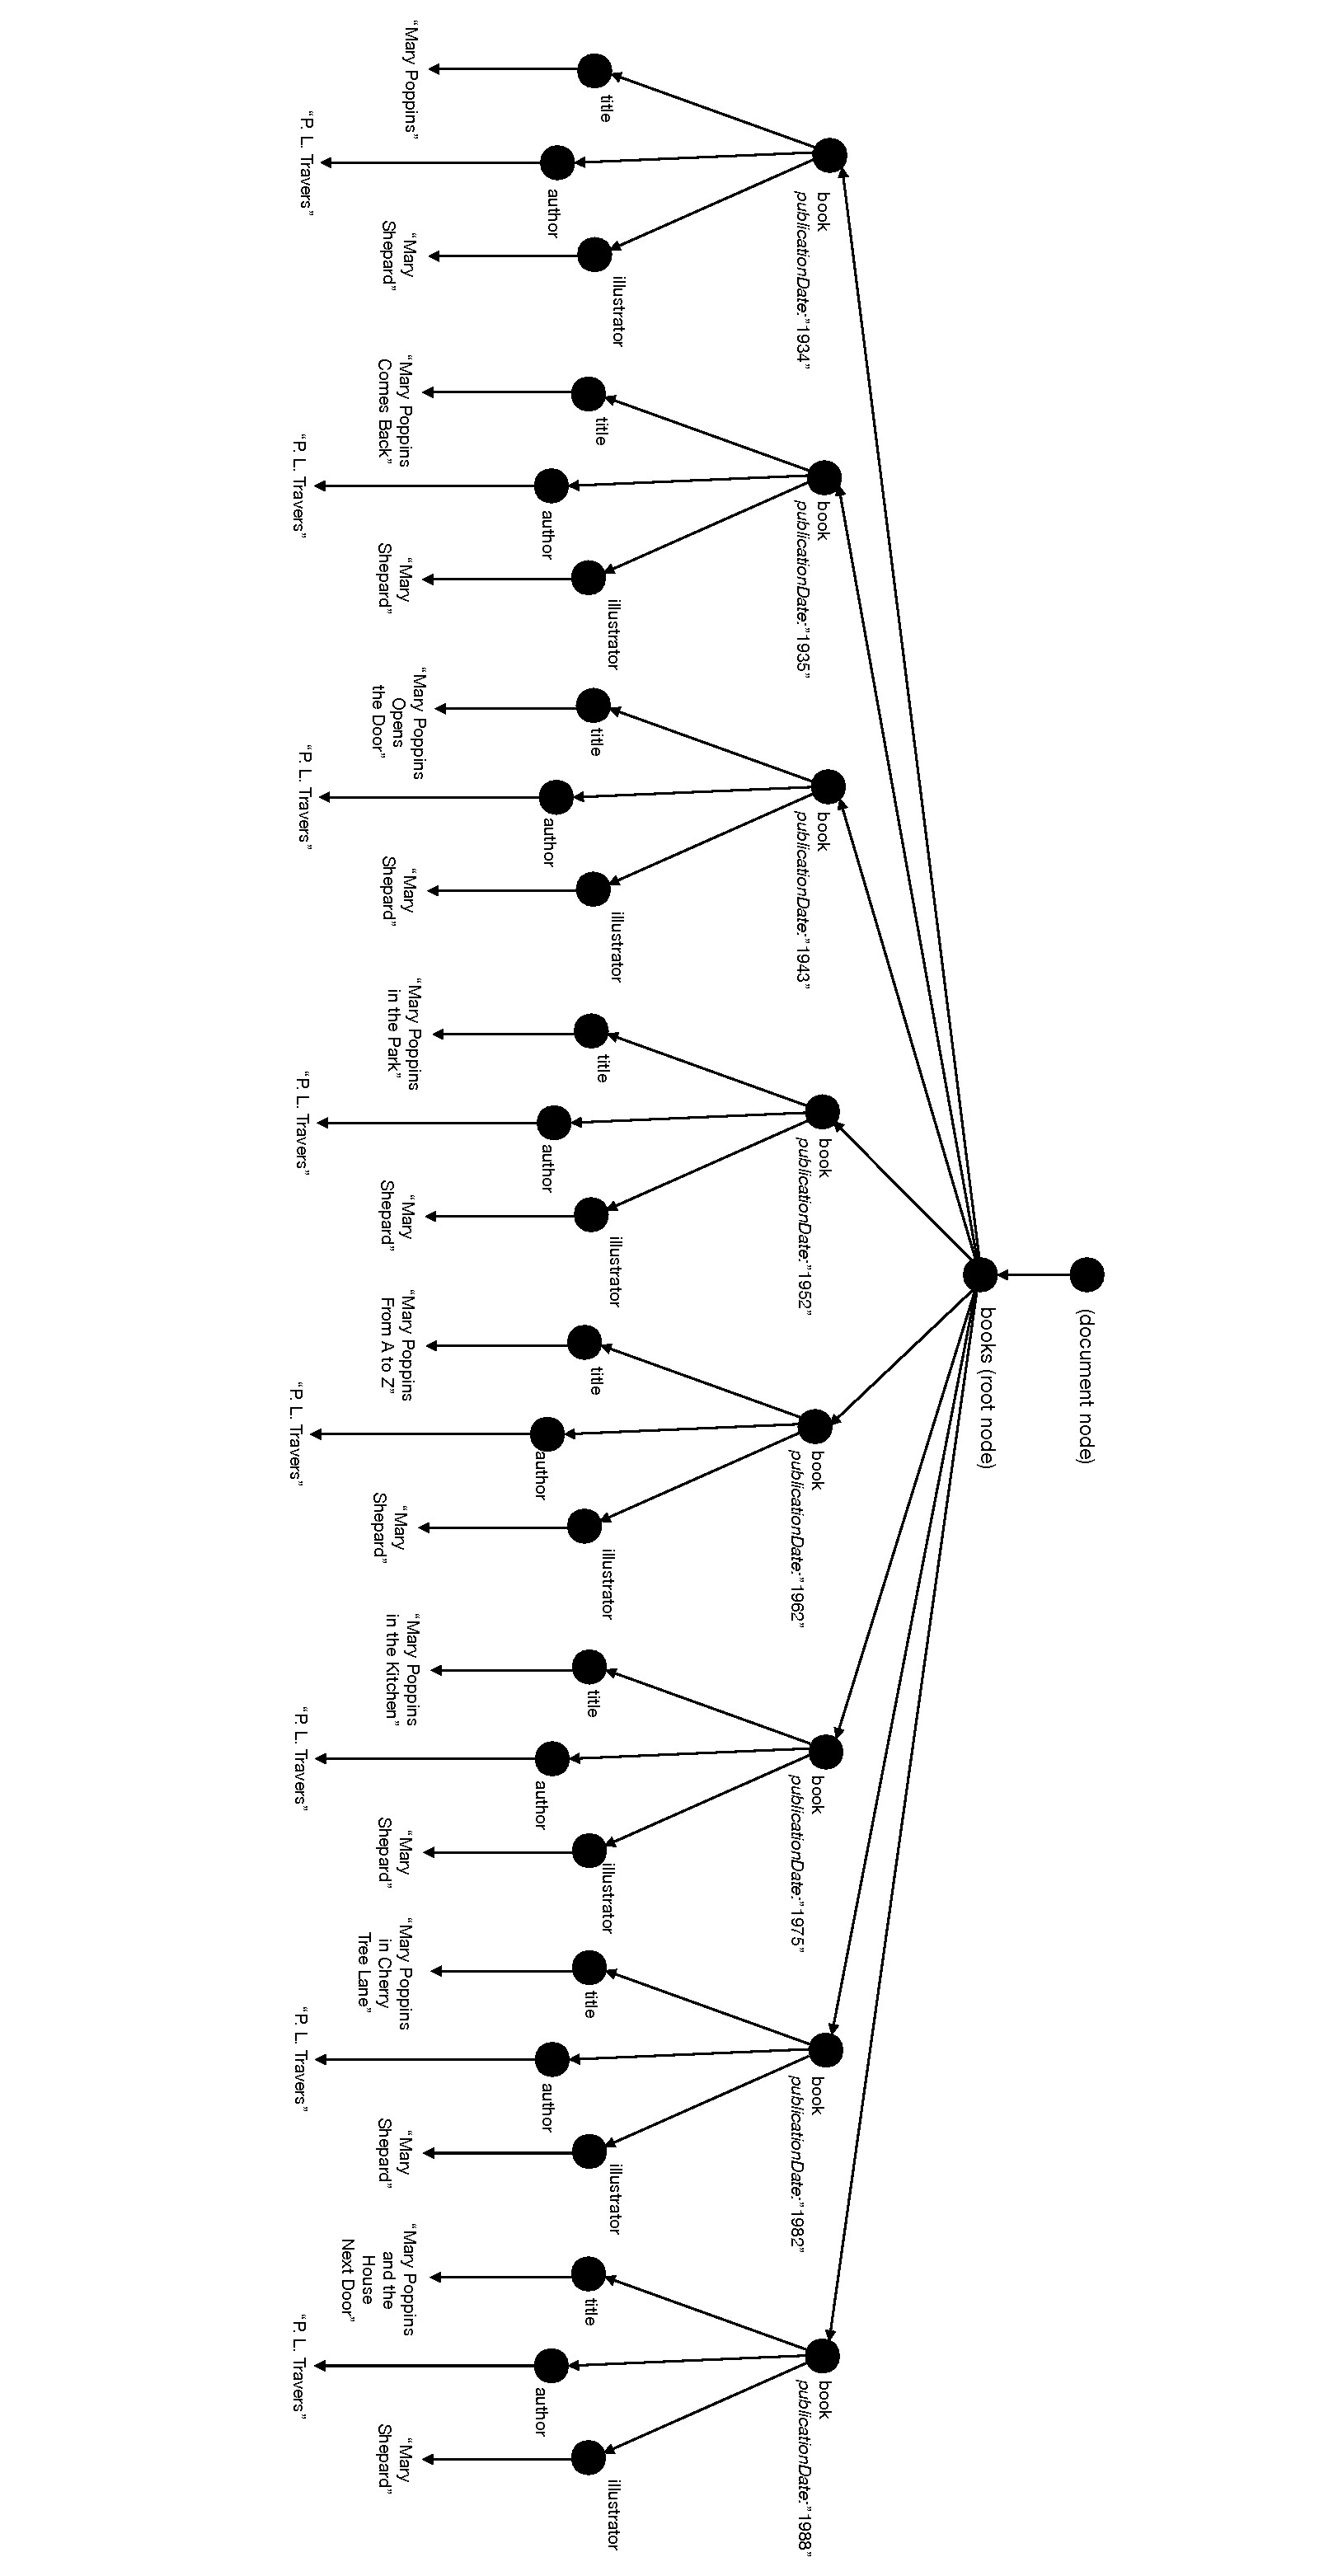
\includepdf[pages=-]{diagram.pdf}


\end{document}